\documentclass[../dissertation.tex]{subfiles}
\begin{appendices}

\chapter{Additional Information}

\section{MoSCoW Requirements}
\label{sec:moscow}

After defining the scope of the project in Section \ref{sec:scope}, the below MoSCoW requirements \cite{moscowreq} were made. 

Must Have:
\begin{itemize}
    \item \textbf{A web endpoint that calls the Tulip Python API.}
	\item \textbf{To be able to deal with large data.} This data must be too large to easily send over the network and be visualised by the client without manipulation.
	\item \textbf{A basic interface to show how the product works.}
	\item \textbf{Data that can be rendered must be  returned from the endpoint.}
\end{itemize}

Should Have:
\begin{itemize}
    \item \textbf{A neat JavaScript client.} Neat is defined as a well-documented list of functions that the client can call that then make calls to the web end-point
	\item \textbf{A flexible web endpoint.} Flexible is defined as covering as many relevant API calls as possible, and making sure that as few of the parameters for the API calls are hard-coded. This has the benefit of both:
	\begin{itemize}
	    \item Making the system more useful for a larger number of clients
        \item Letting users make more than just a JavaScript client, so if they want to make a C\# or Java app that would not create a problem
	\end{itemize}
\end{itemize}
	
Could Have:
\begin{itemize}
    \item \textbf{The ability to ask for an image to be returned if client is low power} This would mean that the visualisation would not be interactive, but would take very little time to transfer the image and next to no time to render it, as opposed to far more time for both tasks to send a network to be constructed on the client.
	\item \textbf{The ability for a user to link their hosted data to the application} This could be an in-house solution such as a a company network storage, or an external data host such as Amazon's S3 \cite{amazons3}. Hence, big data (hundreds of gigabytes or terrabytes) could be linked to the system with ease, each one being imported and linked to the system manually, or an XML/JSON file could be provided that allowed for batch uploading of data. 
\end{itemize}
	
Won't have but would like:
\begin{itemize}
    \item \textbf{A fully fledged and pretty interface.} It would be nice to have a fully completed front-end that is very user-friendly and has been thoroughly evaluated and tested. However, given the amount of time available for the project, it was decided that this is not as critical as having back-end functionality, and additionally that the front-end is being created to demonstrate what the back-end can do as much as to be part of the project.
\end{itemize}

\section{Technical Infrastructure Sketch}
\label{sec:tech_infra_app}

See Figure \ref{fig:techinfra_app} for first draft of the technical infrastructure.

\begin{figure}[H]
    \centering
    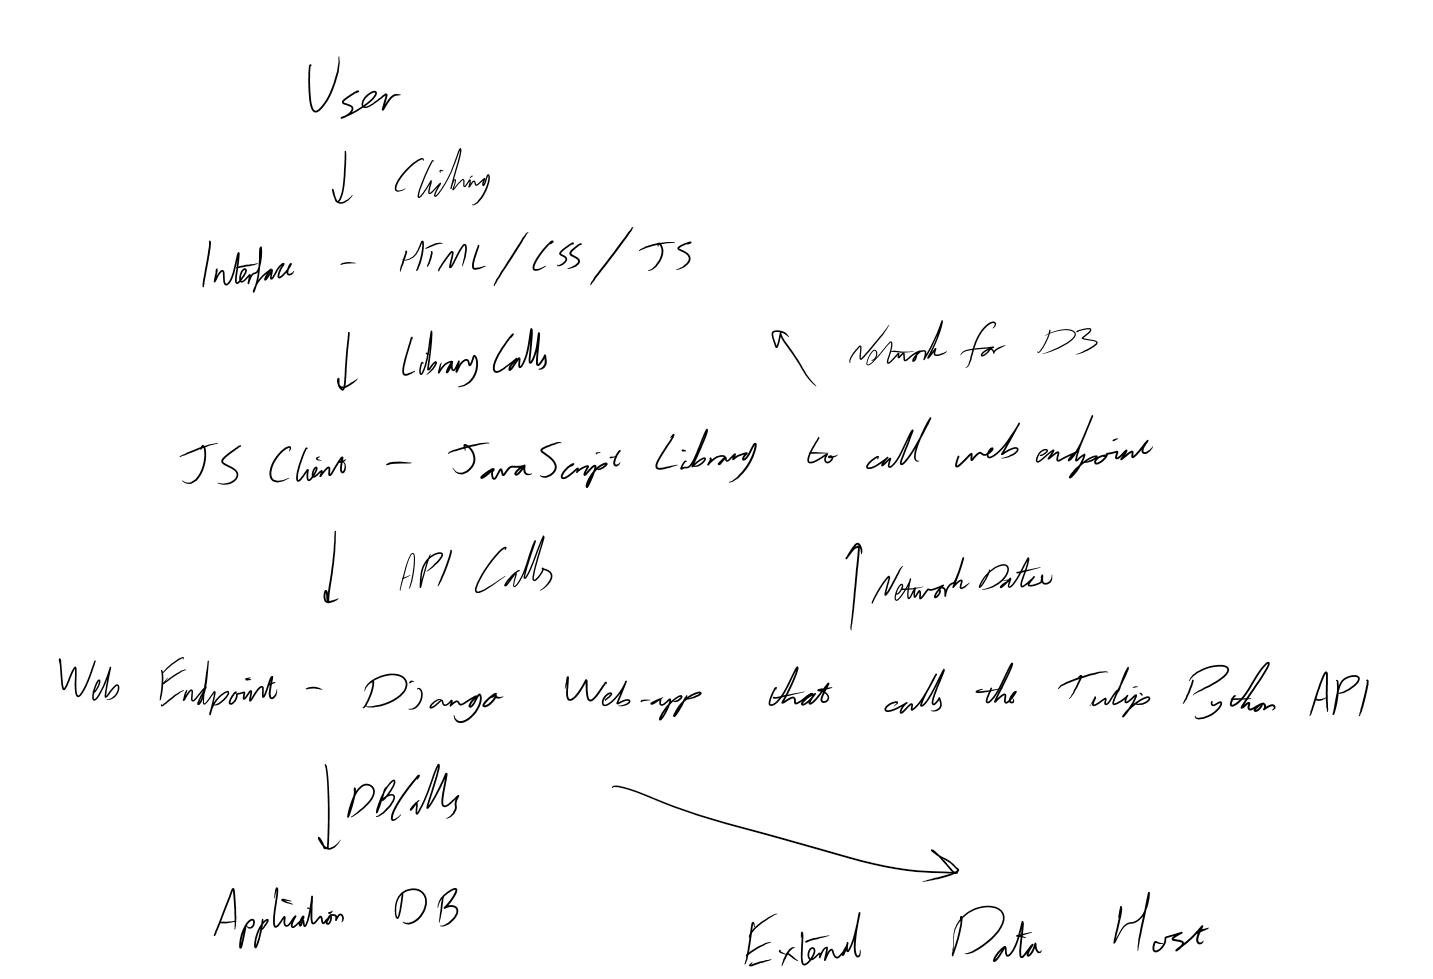
\includegraphics[width=17cm]{6/tech_infra}
    \caption{Draft of Technical Infrastructure}
    \label{fig:techinfra_app}
\end{figure}

\section{What is Hadoop?}
\label{sec:whatishadoop}

Hadoop is a set of open source programs that contain four core modules. These are:

\begin{itemize}
    \item Hadoop Common: The common utilities that support the other Hadoop modules.
    \item Hadoop Distributed File System (HDFS™): A distributed file system that provides high-throughput access to application data.
    \item Hadoop MapReduce: A YARN-based system for parallel processing of large datasets.
    \item Hadoop YARN: A framework for job scheduling and cluster resource management.
\end{itemize}

These combine to give a way of storing, scheduling and processing Big Data in parallel. The way Hadoop could be utilised by the developed application is by storing all of the data that is to be visualised on HDFS. This would be done by using YARN to schedule the node and edge bundling jobs and then manage the resources available to the cluster where the jobs would be run. Next, MapReduce would be used to process each of the sub-networks and finally combine them back into a single network.

%------------------------------------------------------------

\chapter{Full Performance Evaluation Results}
\label{sec:perf-eval-tab}

The below tables - Table \ref{table:30-nodes-full}, \ref{table:200-nodes-full}, \ref{table:1000-nodes-full}, \ref{table:3000-nodes-full} - show the average of five runs collecting: how long different parts of the process took, the total time standard deviation, the number of edges and nodes, and the packet size.

\begin{table}[ht]
\centering
\begin{tabular}{|l|l|l|l|l|}
\hline
                                   & \textbf{None}  & \textbf{Edge-based Bundling}  & \textbf{Pruning} & \textbf{Both} \\ \hline
Time from click to AJAX response   & 12.4  & 17    & 15.6    & 15.8 \\ \hline
Time spend processing in Vis.js    & 0.8   & 0.8   & 0.6     & 0.6  \\ \hline
Time spend creating vis.js network & 22.2  & 20.8  & 12.6    & 9    \\ \hline
Time spend drawing                 & 135.2 & 91    & 57      & 37.8 \\ \hline
Sum of all JS times                & 170.6 & 129.6 & 85.8    & 63.2 \\ \hline
Time from first to last Date()     & 170.8 & 129.6 & 85.8    & 63.2 \\ \hline
Total Time Standard Deviation      & 15.2  & 19.3  & 20.5    & 15.1 \\ \hline
Number of nodes                    & 31    & 18    & 9       & 7    \\ \hline
Number of edges                    & 26    & 13    & 4       & 2    \\ \hline
Time to load in the TLP            & 0.64  & 0.7   & 0.8     & 0.72 \\ \hline
Time to prune the network          &       &       & 0.38    & 0.32 \\ \hline
Time to bundle on edges            &       & 0.36  &         & 0.1  \\ \hline
Packet Size                        & 1300  & 1012  & 827     & 785  \\ \hline
\end{tabular}
\caption{31 Nodes}
\label{table:30-nodes-full}
\end{table}

\begin{table}[ht]
\centering
\begin{tabular}{|l|l|l|l|l|}
\hline
                                   & \textbf{None}  & \textbf{Edge-based Bundling}  & \textbf{Pruning} & \textbf{Both} \\ \hline
Time from click to AJAX response   & 50     & 20.2   & 22      & 19    \\ \hline
Time spend processing in Vis.js    & 4      & 3.6    & 2.2     & 1     \\ \hline
Time spend creating vis.js network & 97.2   & 90     & 44.8    & 23.6  \\ \hline
Time spend drawing                 & 7231.6 & 6635.2 & 593.2   & 102.8 \\ \hline
Sum of all JS times                & 7382.8 & 6749   & 662.2   & 146.4 \\ \hline
Time from first to last Date()     & 7382.8 & 6749   & 663     & 146.6 \\ \hline
Total Time Standard Deviation      & 2010.2 & 1074.9 & 187     & 14.5  \\ \hline
Number of nodes                    & 199    & 155    & 60      & 17    \\ \hline
Number of edges                    & 199    & 155    & 60      & 17    \\ \hline
Time to load in the TLP            & 1.24   & 1.2    & 1.18    & 1.16  \\ \hline
Time to prune the network          &        &        & 2.86    & 2.52  \\ \hline
Time to bundle on edges            &        & 1.4    &         & 0.6   \\ \hline
Packet Size                        & 7600   & 6100   & 3900    & 2300  \\ \hline
\end{tabular}
\caption{199 Nodes}
\label{table:200-nodes-full}
\end{table}

\begin{table}[ht]
\centering
\begin{tabular}{|l|l|l|l|l|}
\hline
                                   & \textbf{None}  & \textbf{Edge-based Bundling}  & \textbf{Pruning} & \textbf{Both} \\ \hline
Time from click to AJAX response   & 177.4   & 126.6   & 58.8    & 57    \\ \hline
Time spend processing in Vis.js    & 15      & 13.4    & 9.2     & 2.6   \\ \hline
Time spend creating vis.js network & 361.2   & 242.2   & 108.2   & 16.2  \\ \hline
Time spend drawing                 & 59370.8 & 37757.6 & 9241.6  & 76.8  \\ \hline
Sum of all JS times                & 59924.4 & 38139.8 & 9417.8  & 152.6 \\ \hline
Time from first to last Date()     & 59925   & 38140.2 & 9418.4  & 152.6 \\ \hline
Total Time Standard Deviation      & 8343.5  & 9383    & 2223.1  & 30.5  \\ \hline
Number of nodes                    & 1089    & 627     & 226     & 12    \\ \hline
Number of edges                    & 1087    & 625     & 224     & 10    \\ \hline
Time to load in the TLP            & 5.32    & 4.72    & 3.44    & 3.28  \\ \hline
Time to prune the network          &         &         & 33.28   & 33.26 \\ \hline
Time to bundle on edges            &         & 13.68   &         & 2.34  \\ \hline
Packet Size                        & 41400   & 29400   & 20300   & 12400 \\ \hline
\end{tabular}
\caption{1089 Nodes}
\label{table:1000-nodes-full}
\end{table}

\begin{table}[ht]
\centering
\begin{tabular}{|l|l|l|l|l|}
\hline
                                   & \textbf{None}  & \textbf{Edge-based Bundling}  & \textbf{Pruning} & \textbf{Both} \\ \hline
Time from click to AJAX response   & 646      & 423      & 314.2   & 241     \\ \hline
Time spend processing in Vis.js    & 35.8     & 33       & 26.8    & 16.8    \\ \hline
Time spend creating vis.js network & 850.4    & 593      & 308.8   & 135.4   \\ \hline
Time spend drawing                 & 251316.6 & 130557.2 & 48306.4 & 14139.6 \\ \hline
Sum of all JS times                & 252848.8 & 131606.2 & 48956.2 & 14532.8 \\ \hline
Time from first to last Date()     & 252849.2 & 131606.6 & 48956.8 & 14532.8 \\ \hline
Total Time Standard Deviation      & 32862    & 3937     & 6031.3  & 3341    \\ \hline
Number of nodes                    & 2849     & 1737     & 802     & 286     \\ \hline
Number of edges                    & 2835     & 1719     & 792     & 276     \\ \hline
Time to load in the TLP            & 162.54   & 50.5     & 11.04   & 7.46    \\ \hline
Time to prune the network          &          &          & 169.06  & 184.72  \\ \hline
Time to bundle on edges            &          & 94.04    &         & 7.32    \\ \hline
Packet Size                        & 114000   & 83500    & 63500   & 42900   \\ \hline
\end{tabular}
\caption{2849 Nodes}
\label{table:3000-nodes-full}
\end{table}

%------------------------------------------------------------

\chapter{Screenshots of the System}

The below screenshots show the system visualising a network of: 30 nodes, 200 nodes, 1000 nodes and 3000 nodes. Each network is shown with no algorithm being applied, node pruning being applied, node bundling based on number of edges being applied, and both node pruning and then node bundling based on number of edges being applied.

Additionally, screenshots containing a highly connected network are shown before and after node bundling based on cliques.

% 30 nodes

\begin{figure}[H]
    \centering
    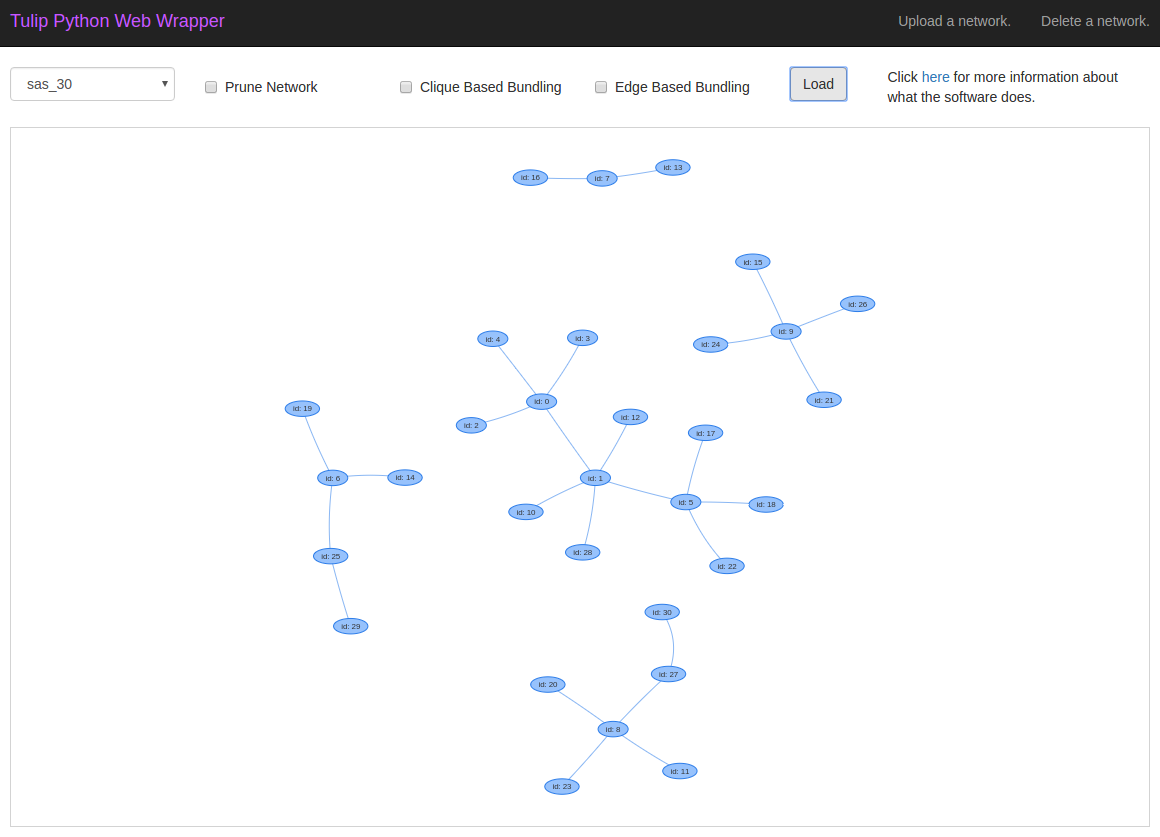
\includegraphics[width=14cm]{appendices/30_1none}
    \caption{This shows a network with 29 nodes being rendered without any algorithm having been applied on the server.}
    \label{fig:30_1none}
\end{figure}

\begin{figure}[H]
    \centering
    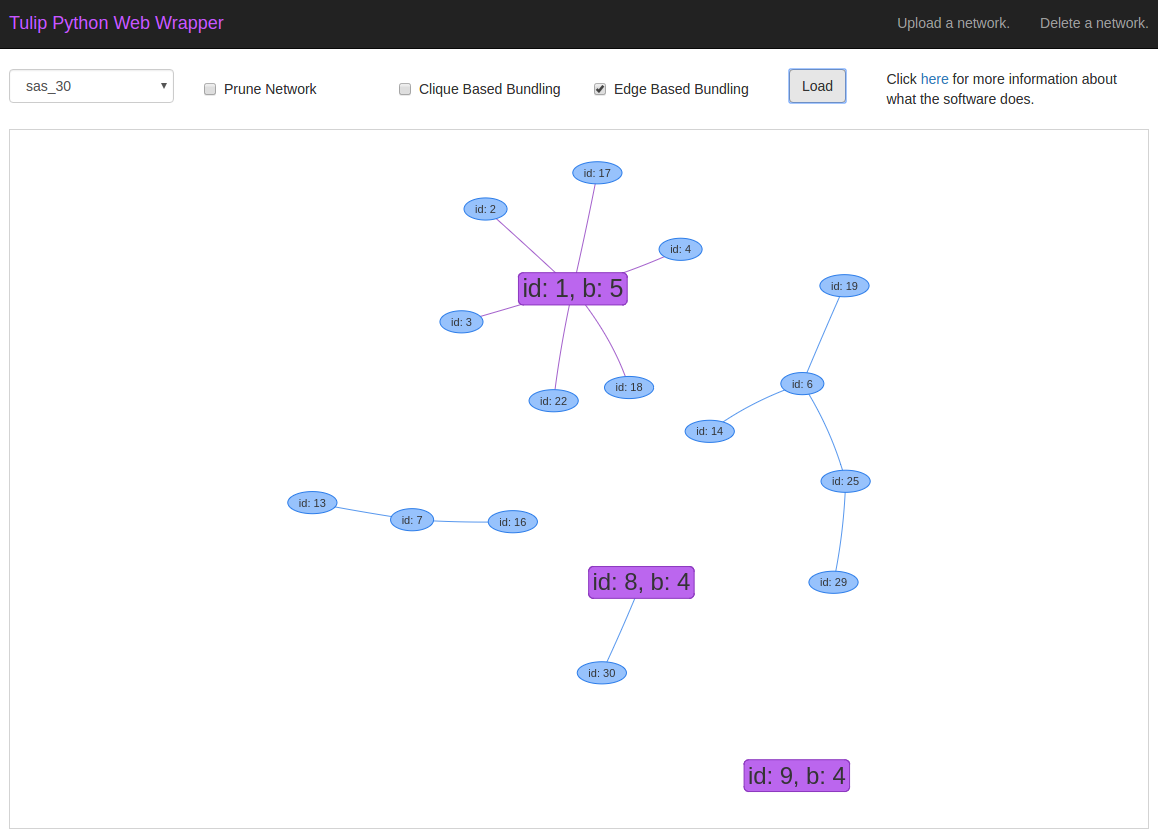
\includegraphics[width=14cm]{appendices/30_2edge}
    \caption{This shows a network with originally 29 nodes being rendered with node bundling based on number of edges.}
    \label{fig:30_2edge}
\end{figure}

\begin{figure}[H]
    \centering
    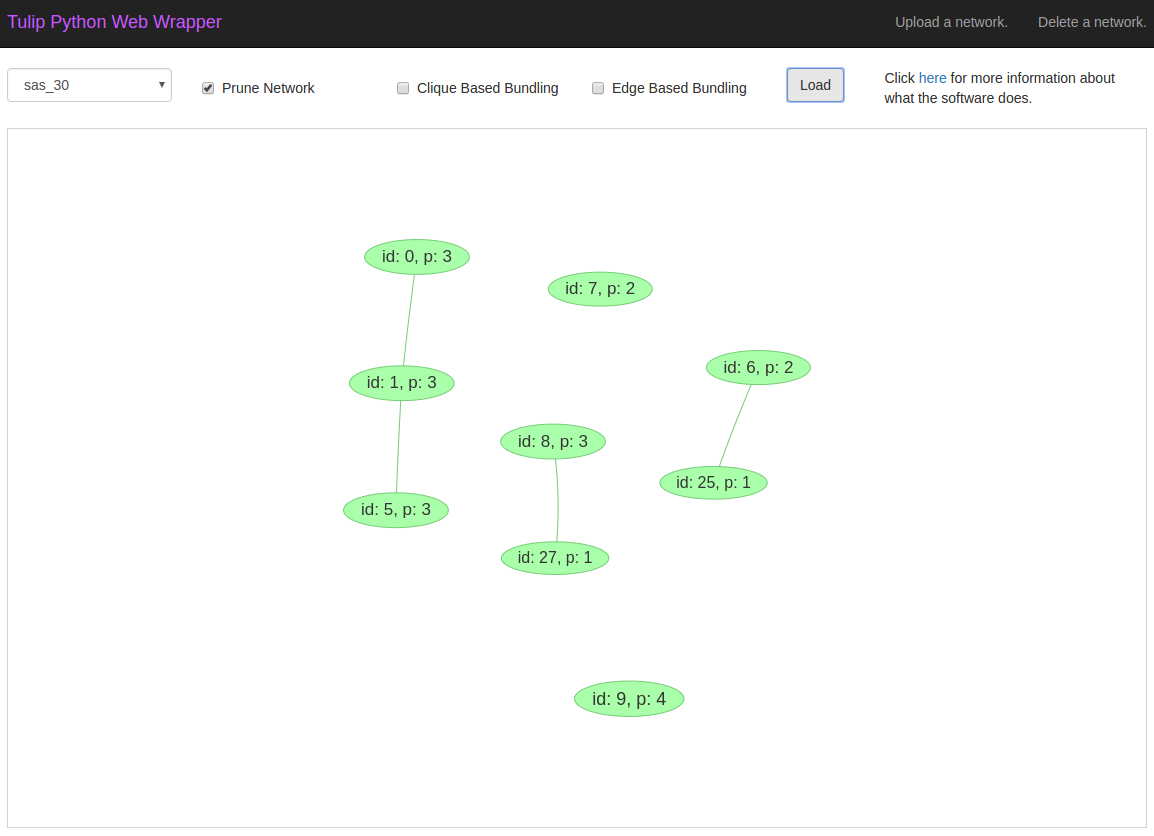
\includegraphics[width=14cm]{appendices/30_3prune}
    \caption{This shows a network with originally 29 nodes being rendered with node pruning.}
    \label{fig:30_3prune}
\end{figure}

\begin{figure}[H]
    \centering
    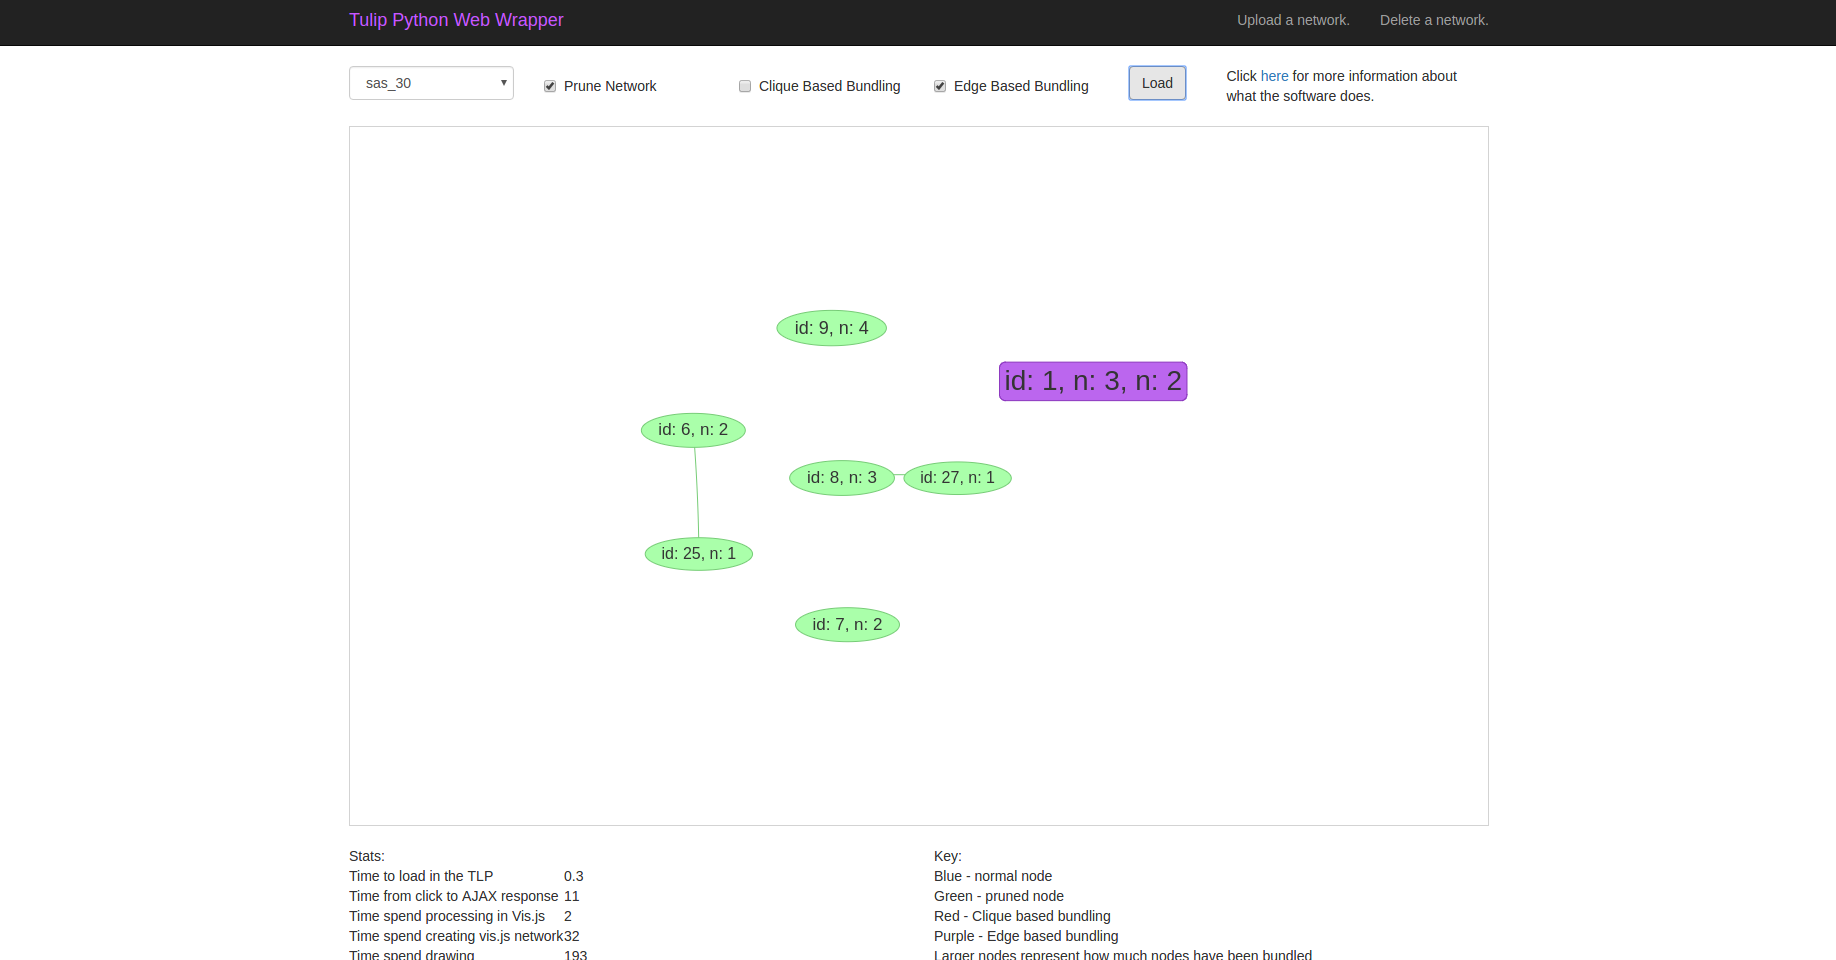
\includegraphics[width=14cm]{appendices/30_4both}
    \caption{This shows a network with originally 29 nodes being rendered with both node pruning and then node bundling based on number of edges.}
    \label{fig:30_4both}
\end{figure}

% 200 nodes

\begin{figure}[H]
    \centering
    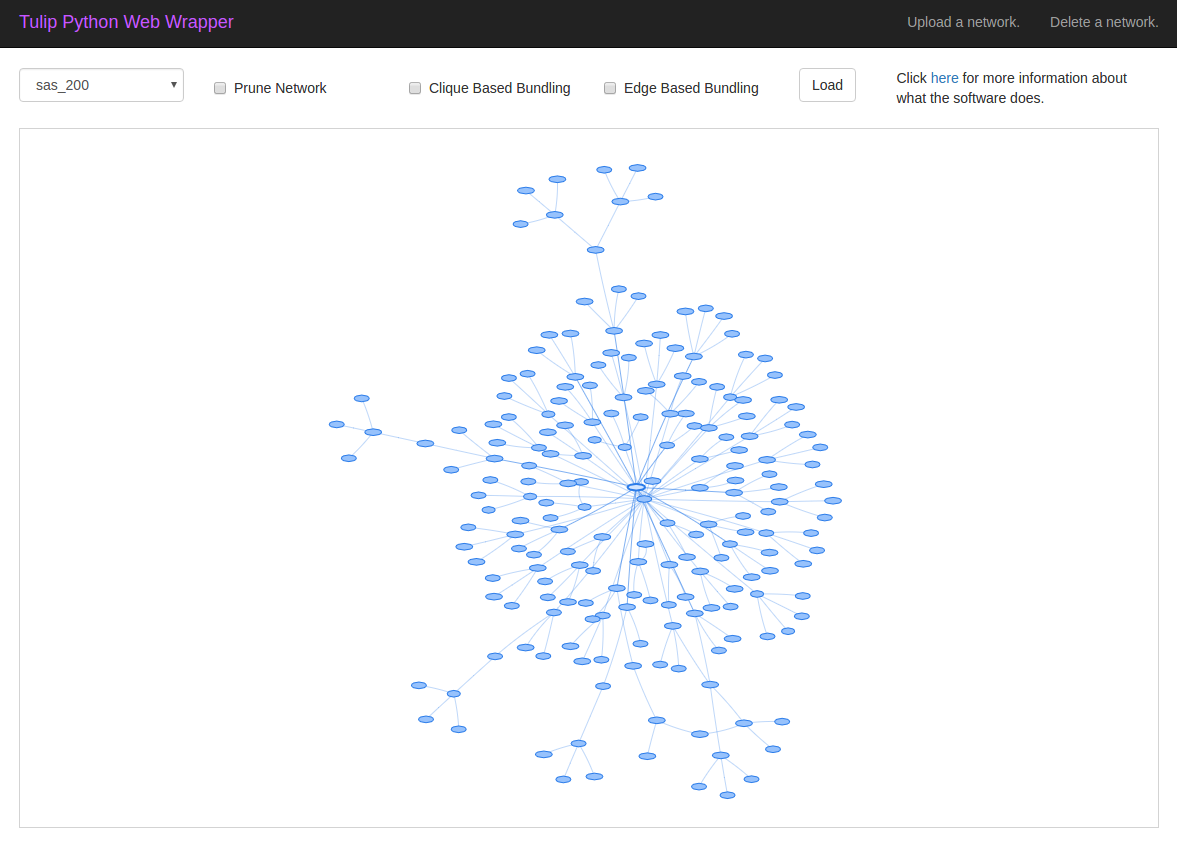
\includegraphics[width=14cm]{appendices/200_1none}
    \caption{This shows a network with 199 nodes being rendered without any algorithm having been applied on the server.}
    \label{fig:200_1none}
\end{figure}

\begin{figure}[H]
    \centering
    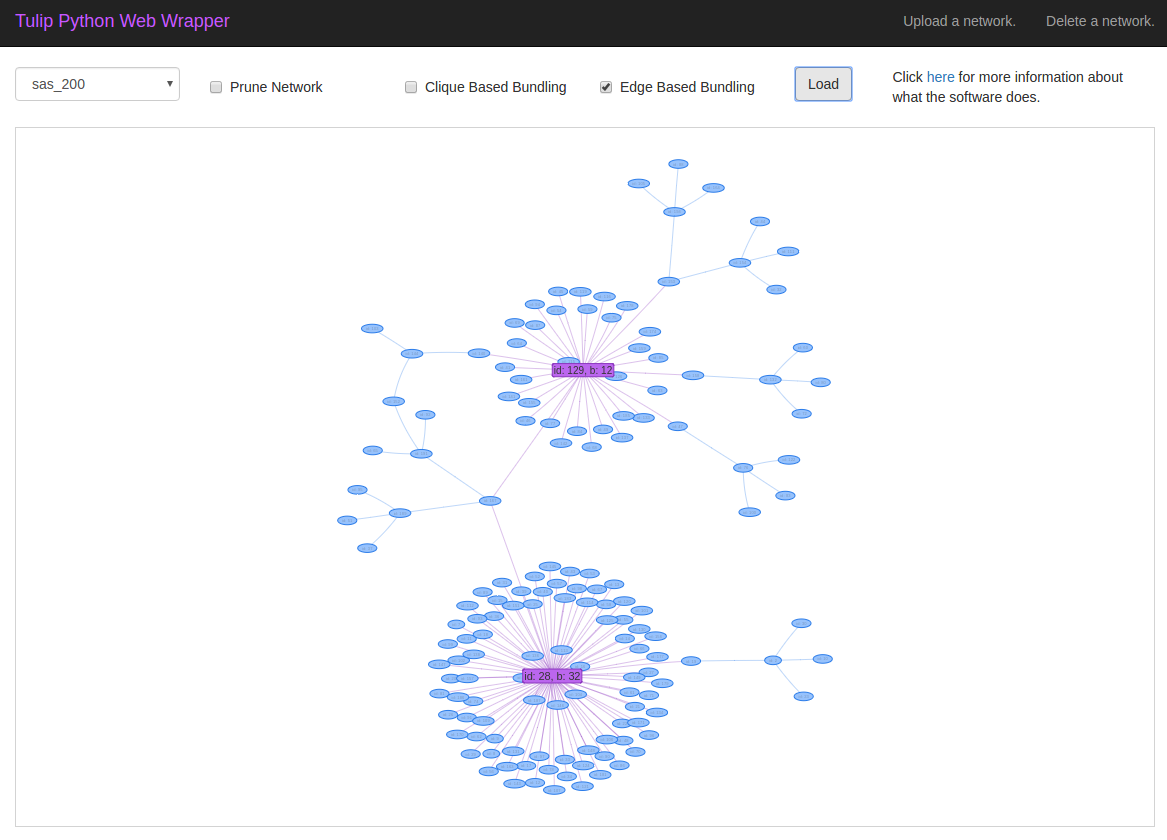
\includegraphics[width=14cm]{appendices/200_2edge}
    \caption{This shows a network with originally 199 nodes being rendered after applying node bundling based on number of edges.}
    \label{fig:200_2edge}
\end{figure}

\begin{figure}[H]
    \centering
    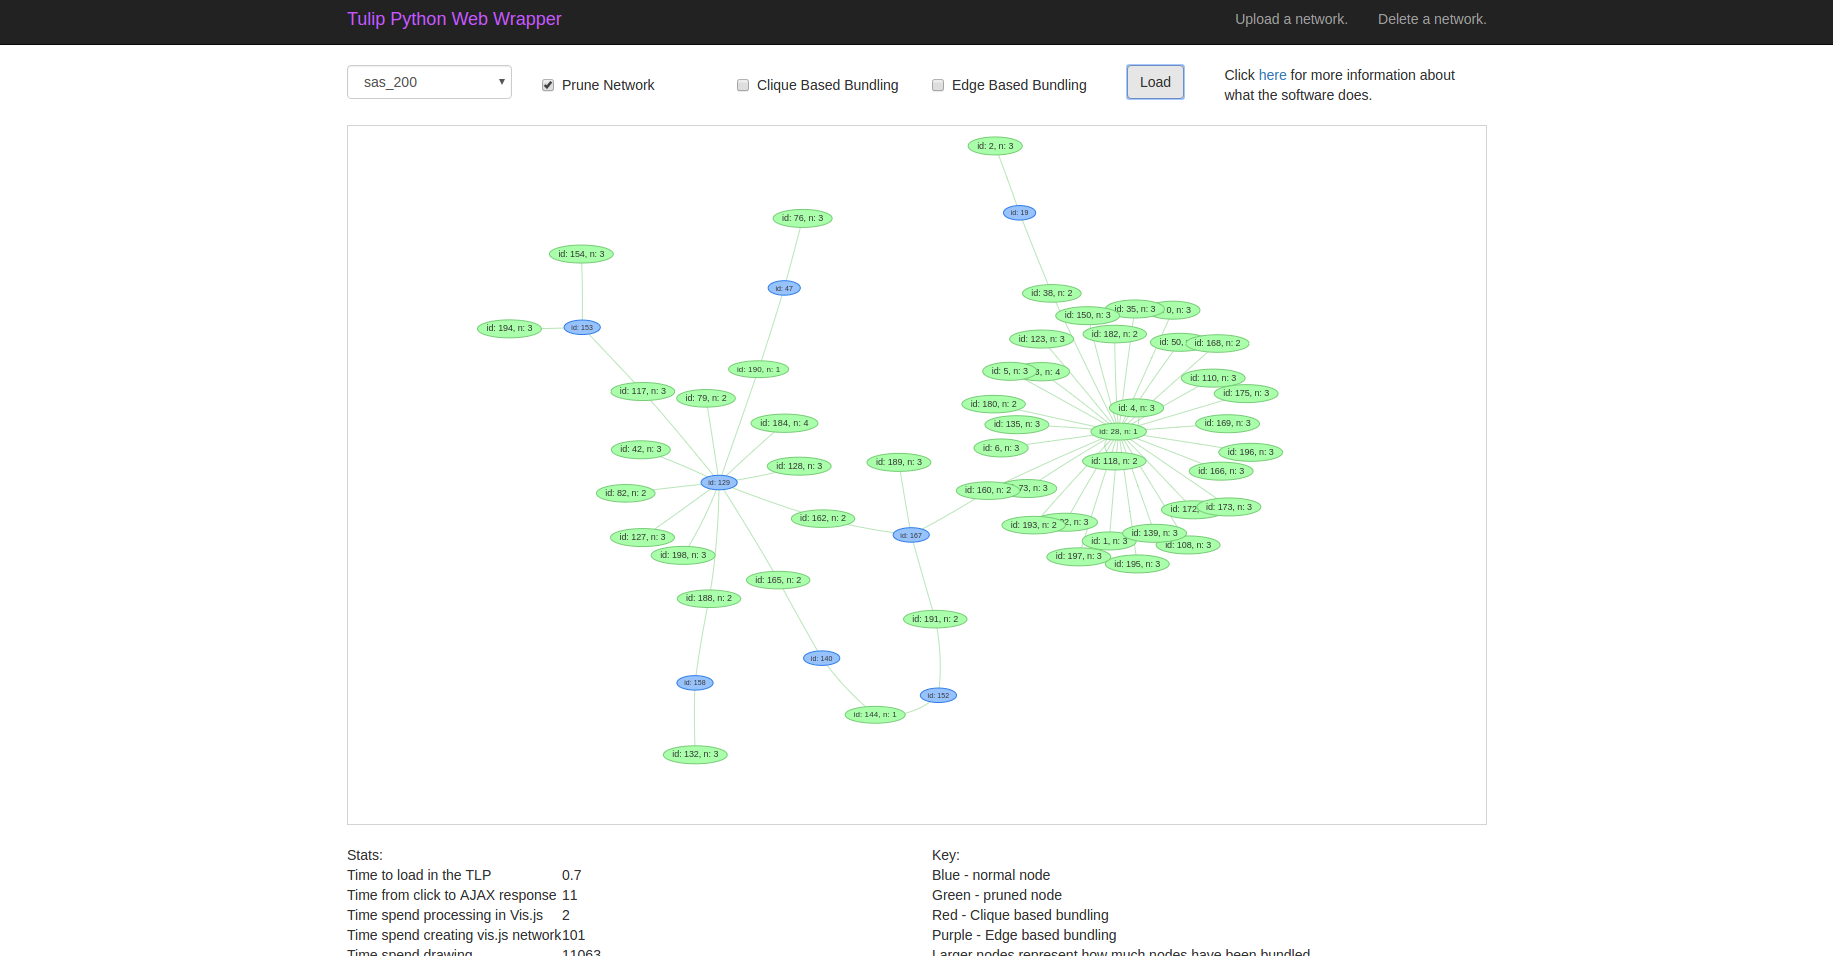
\includegraphics[width=14cm]{appendices/200_3prune}
    \caption{This shows a network with originally 199 nodes being rendered after applying node pruning.}
    \label{fig:200_3prune}
\end{figure}

\begin{figure}[H]
    \centering
    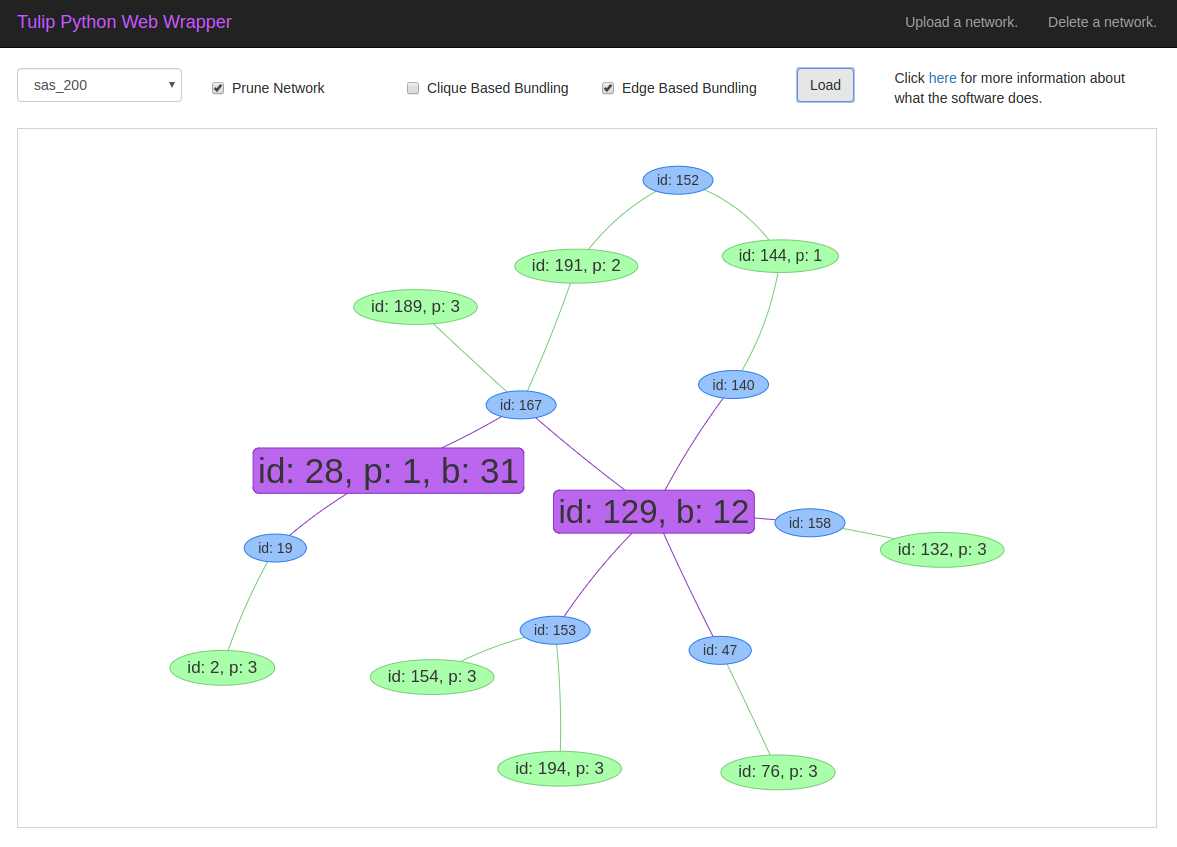
\includegraphics[width=14cm]{appendices/200_4both}
    \caption{This shows a network with originally 199 nodes being rendered after applying both node pruning and then node bundling based on number of edges.}
    \label{fig:200_4both}
\end{figure}

% 1000 nodes

\begin{figure}[H]
    \centering
    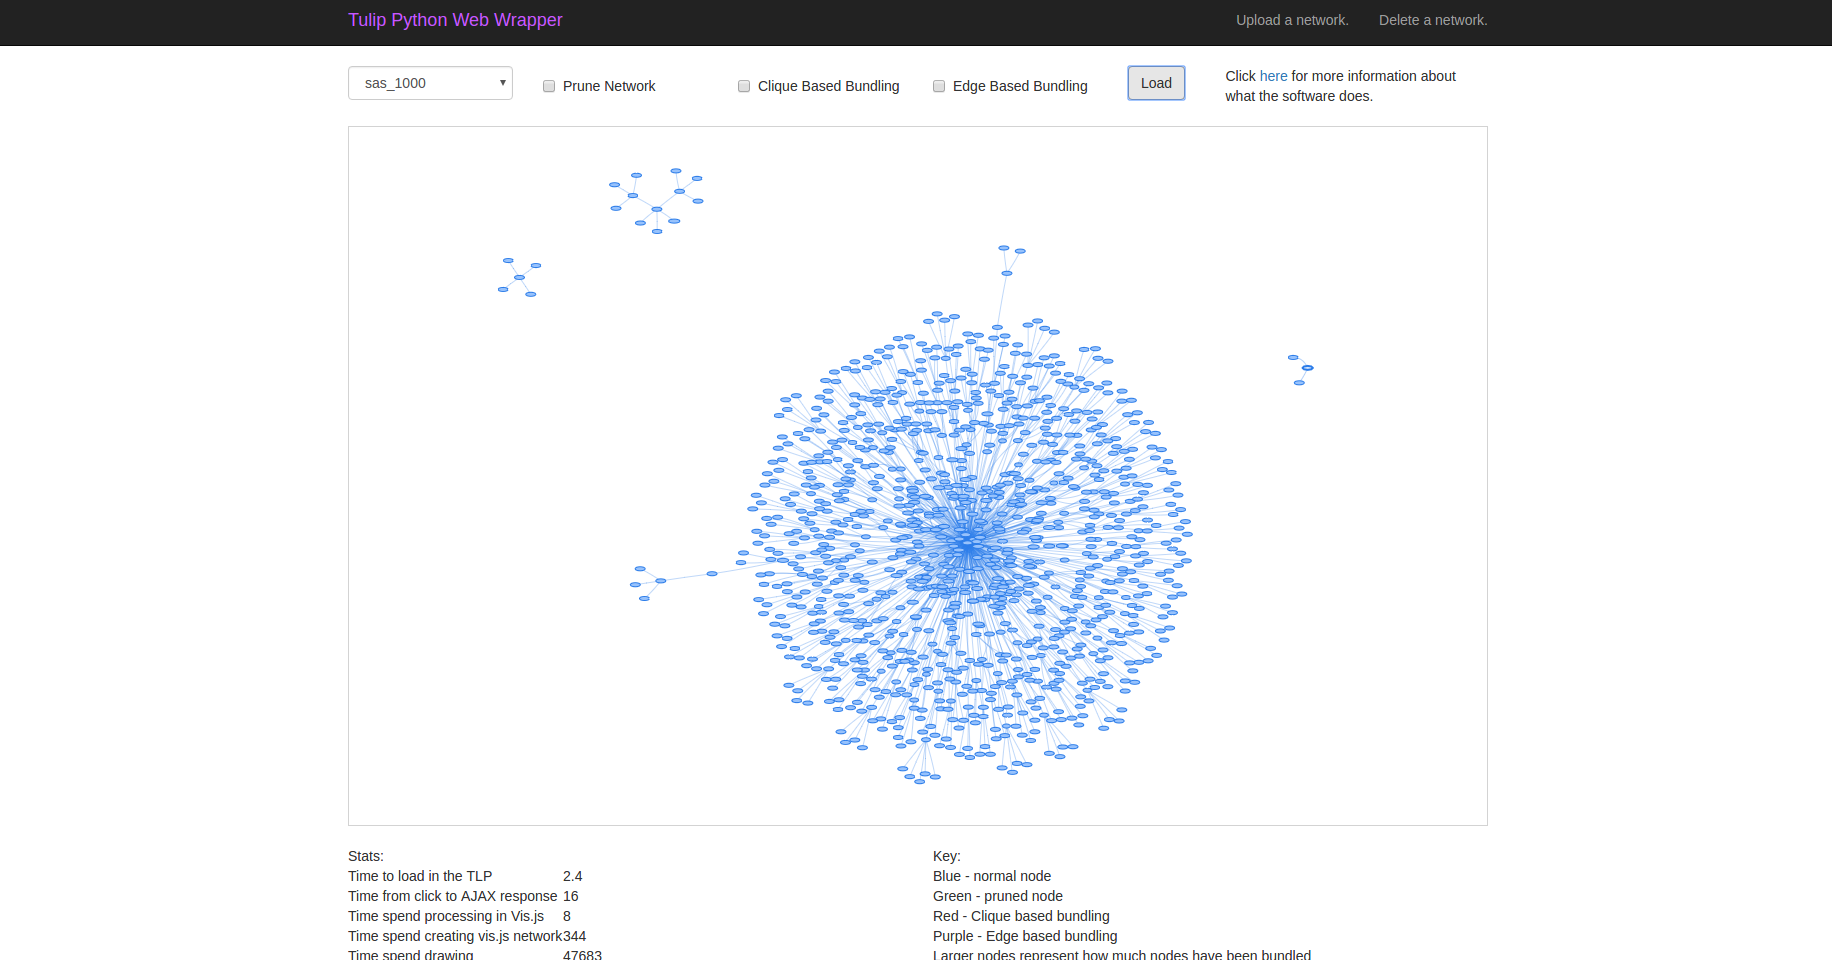
\includegraphics[width=14cm]{appendices/1000_1none}
    \caption{This shows a network with 1089 nodes being rendered without any algorithm having been applied on the server.}
    \label{fig:1000_1none}
\end{figure}

\begin{figure}[H]
    \centering
    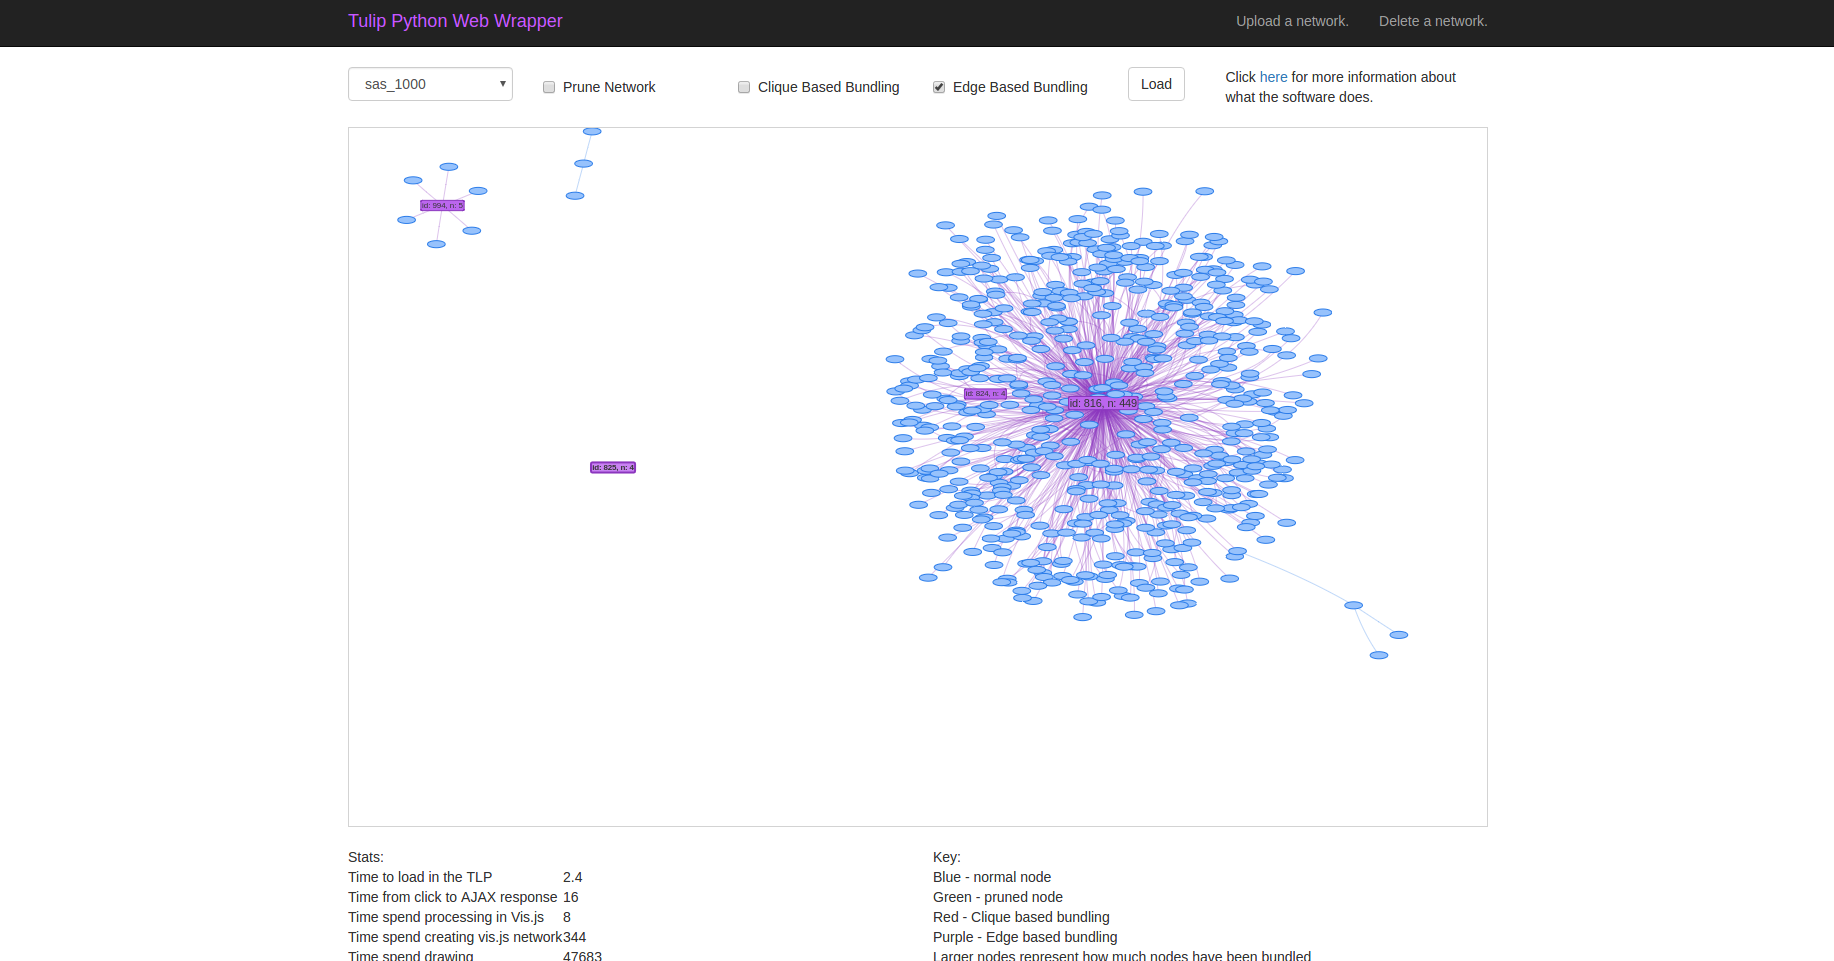
\includegraphics[width=14cm]{appendices/1000_2edge}
    \caption{This shows a network with originally 1089 nodes being rendered after applying node bundling based on number of edges.}
    \label{fig:1000_2edge}
\end{figure}

\begin{figure}[H]
    \centering
    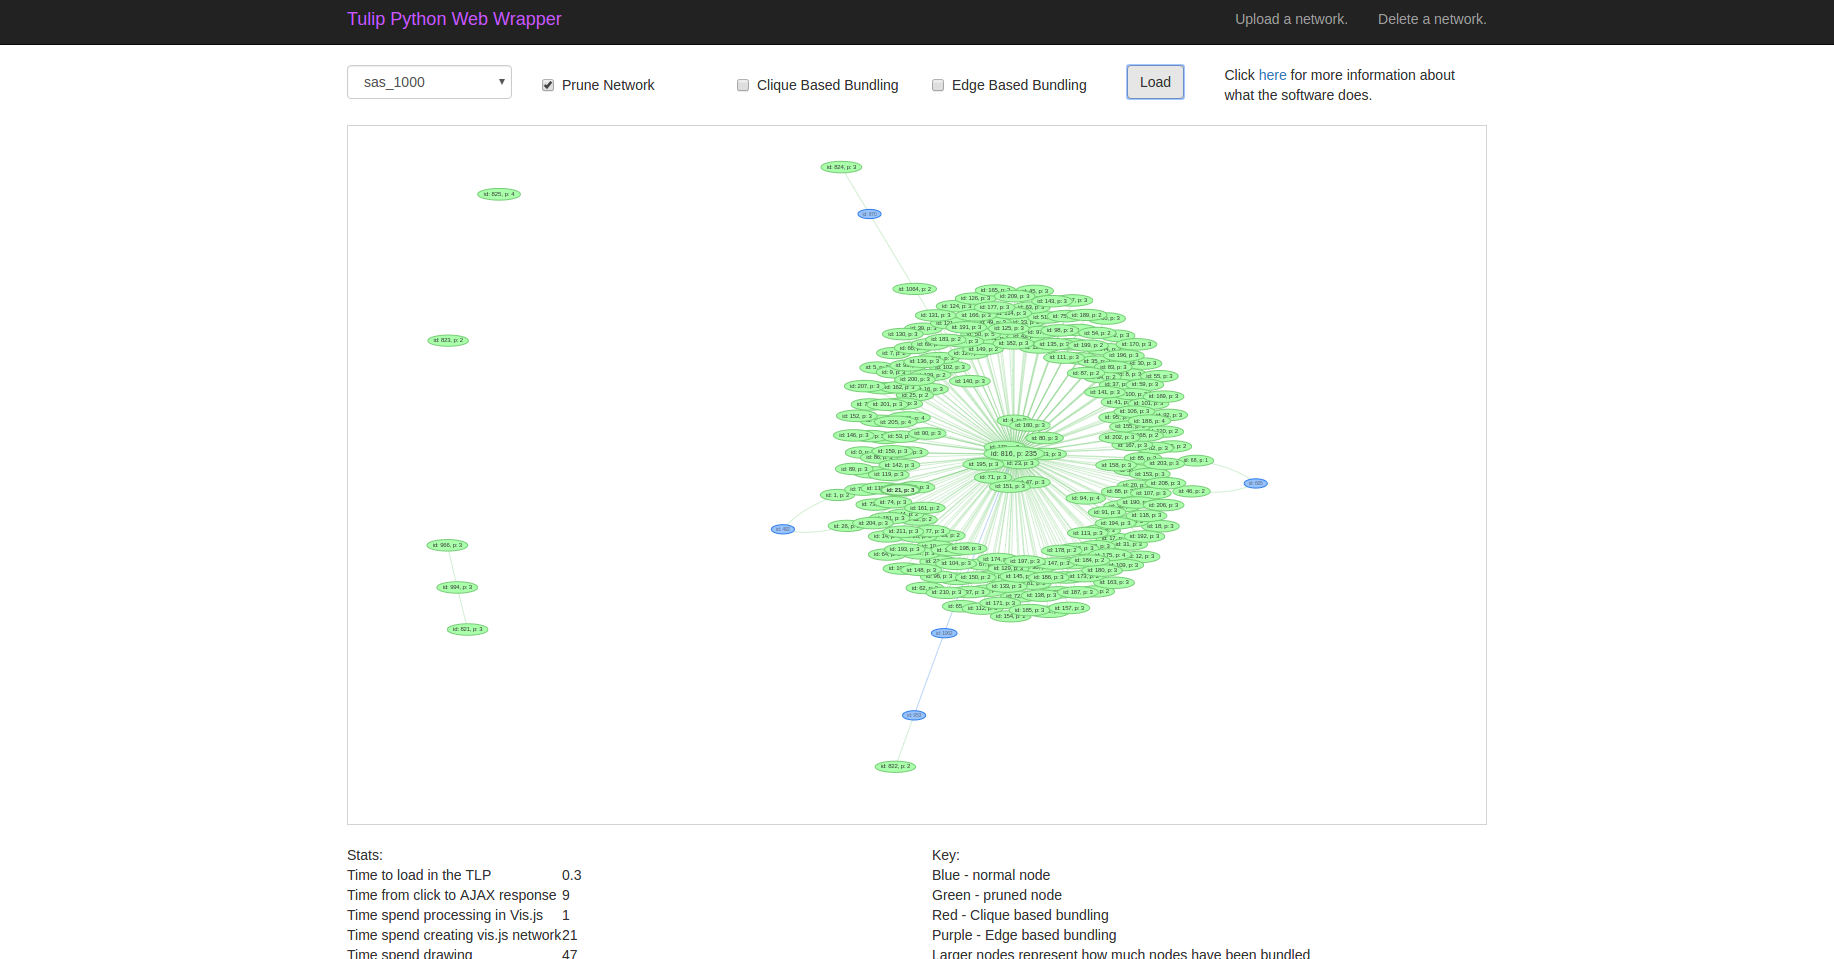
\includegraphics[width=14cm]{appendices/1000_3prune}
    \caption{This shows a network with originally 1089 nodes being rendered after applying node pruning.}
    \label{fig:1000_3prune}
\end{figure}

\begin{figure}[H]
    \centering
    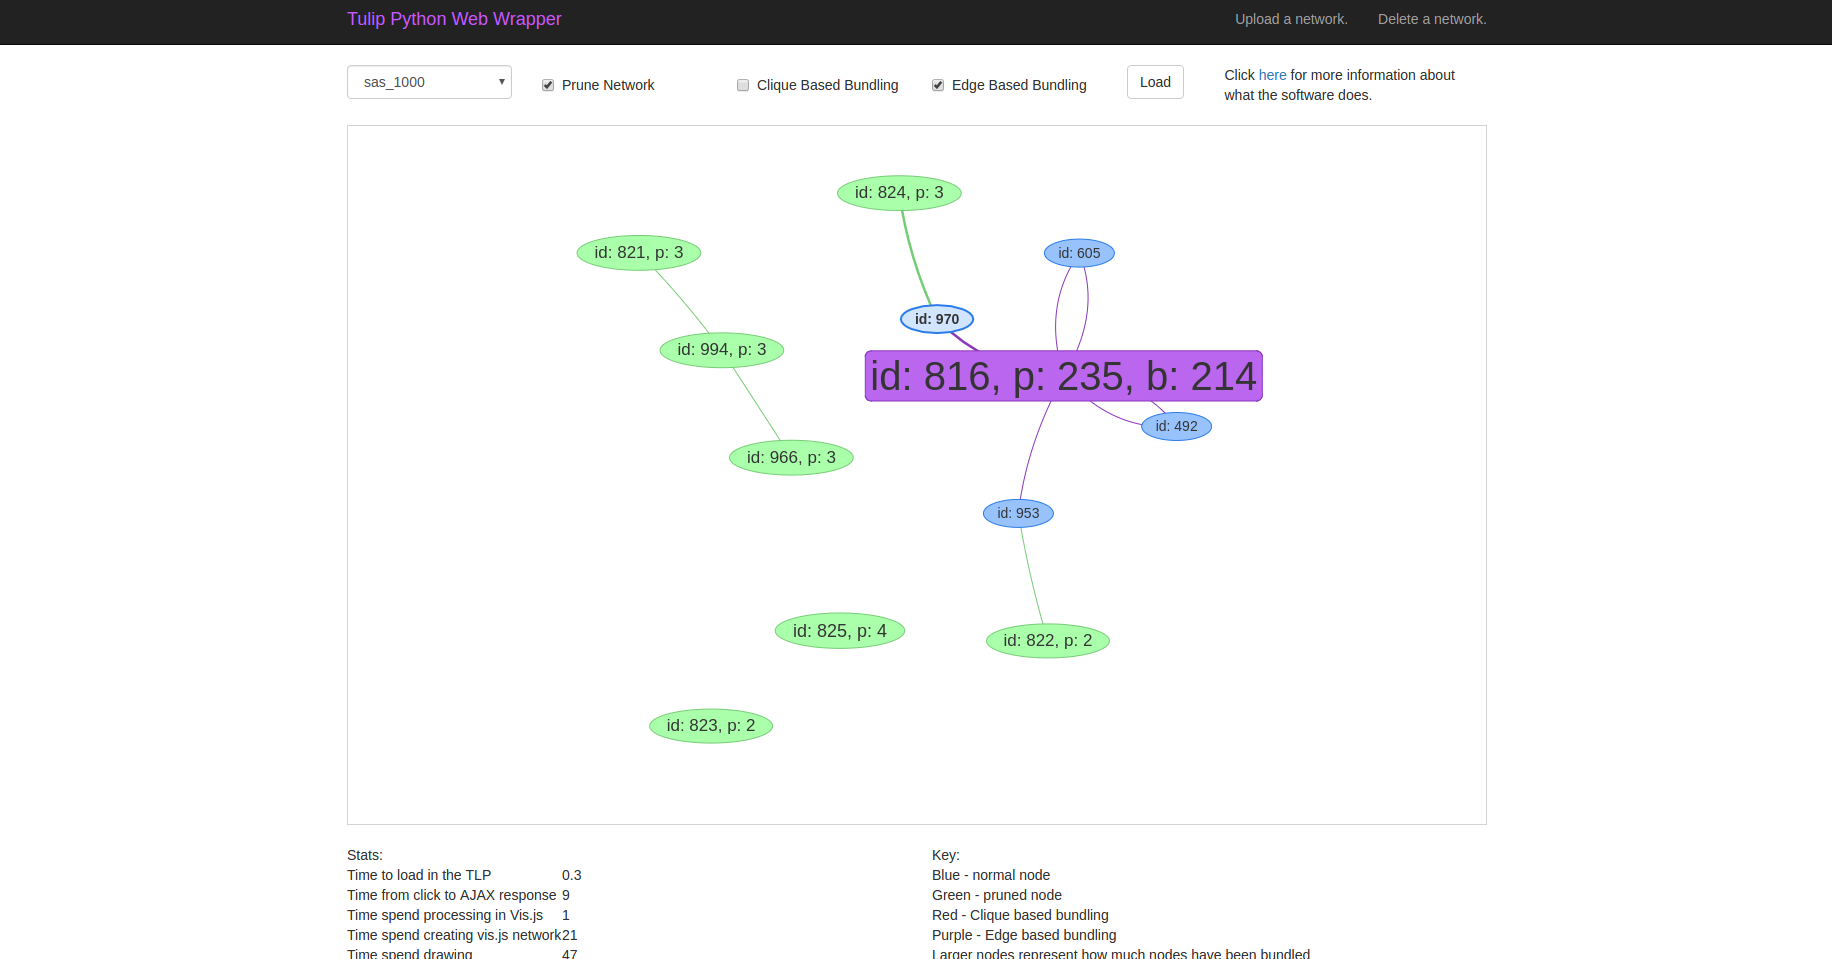
\includegraphics[width=14cm]{appendices/1000_4both}
    \caption{This shows a network with originally 1089 nodes being rendered after applying both node pruning and then node bundling based on number of edges.}
    \label{fig:1000_4both}
\end{figure}

% 3000 nodes

\begin{figure}[H]
    \centering
    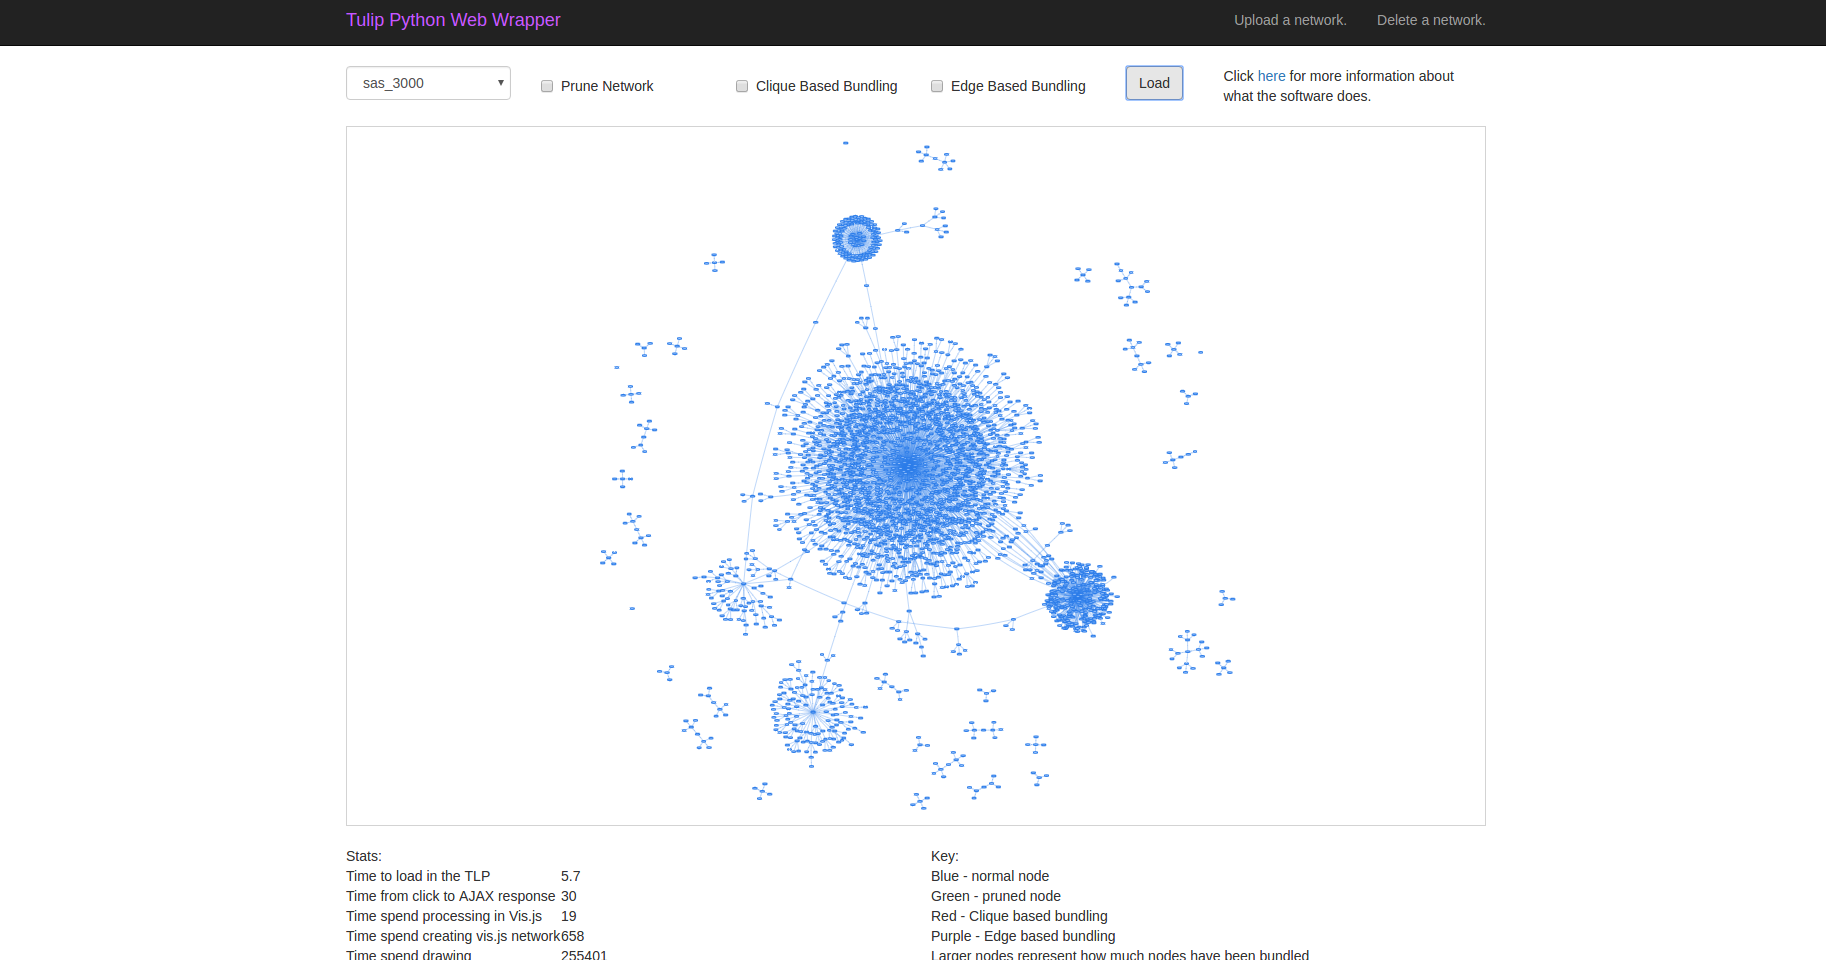
\includegraphics[width=14cm]{appendices/3000_1none}
    \caption{This shows a network with 2849 nodes being rendered without any algorithm having been applied on the server.}
    \label{fig:3000_1none}
\end{figure}

\begin{figure}[H]
    \centering
    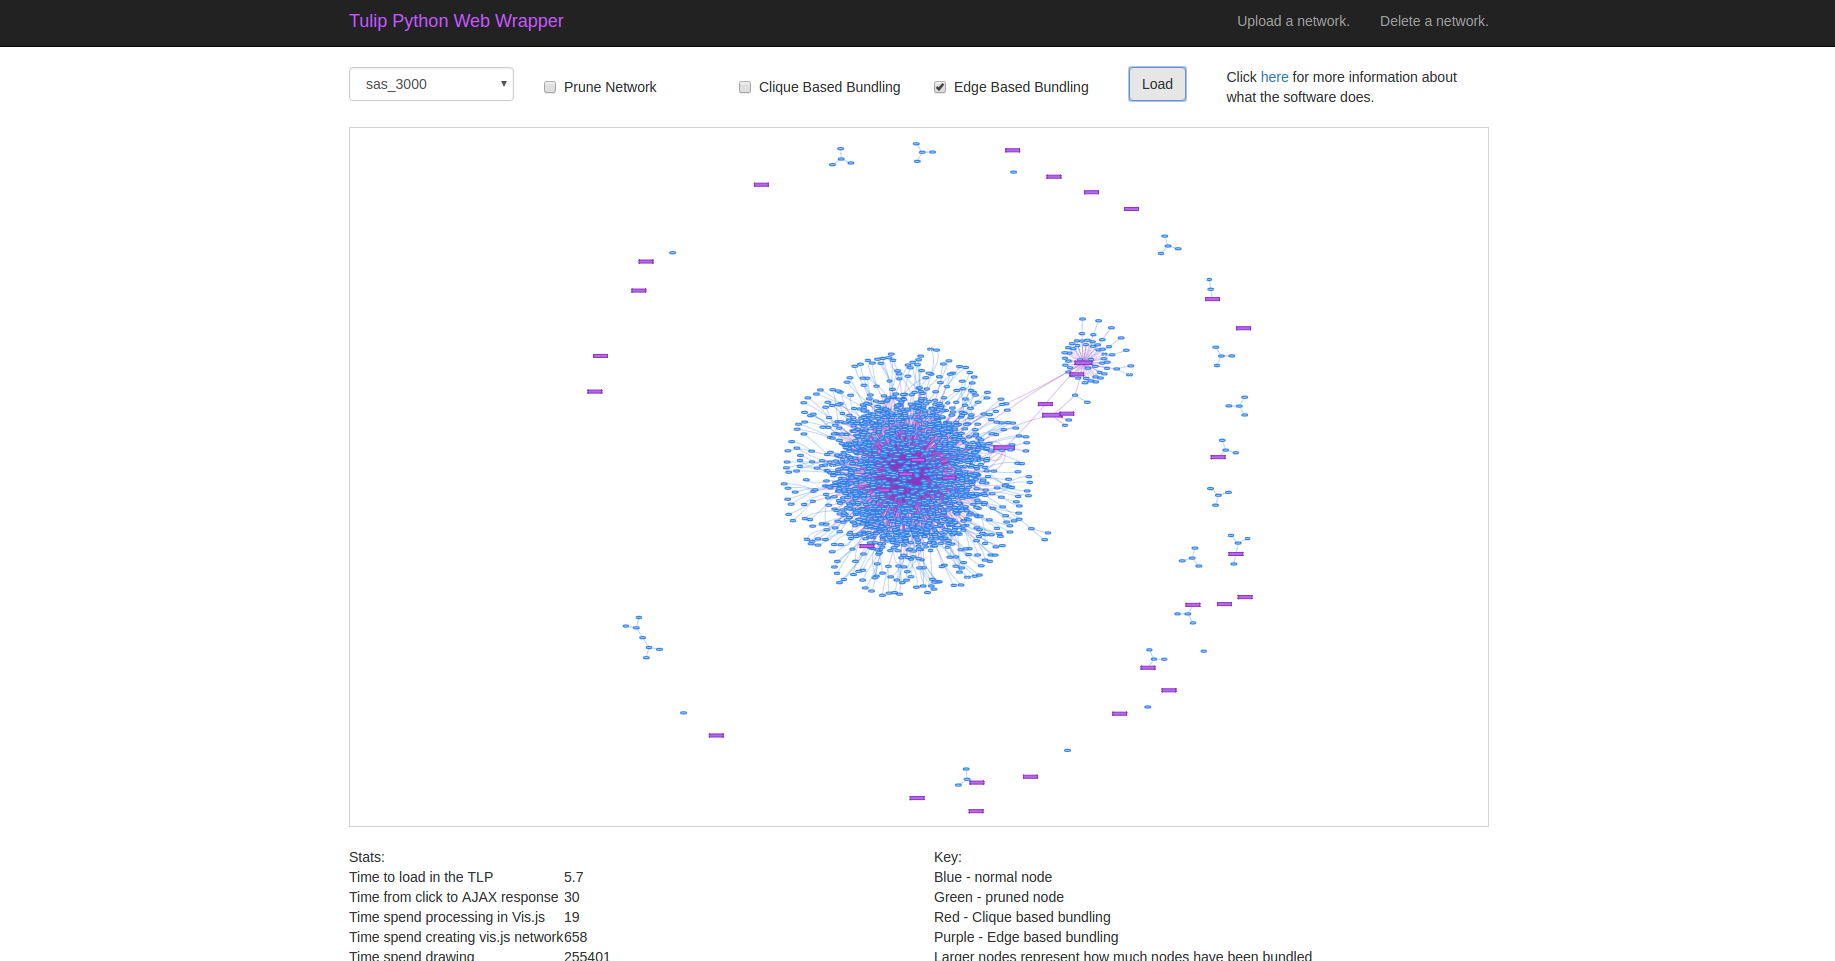
\includegraphics[width=14cm]{appendices/3000_2edge}
    \caption{This shows a network with originally 2849 nodes being rendered after applying node bundling based on number of edges.}
    \label{fig:3000_2edge}
\end{figure}

\begin{figure}[H]
    \centering
    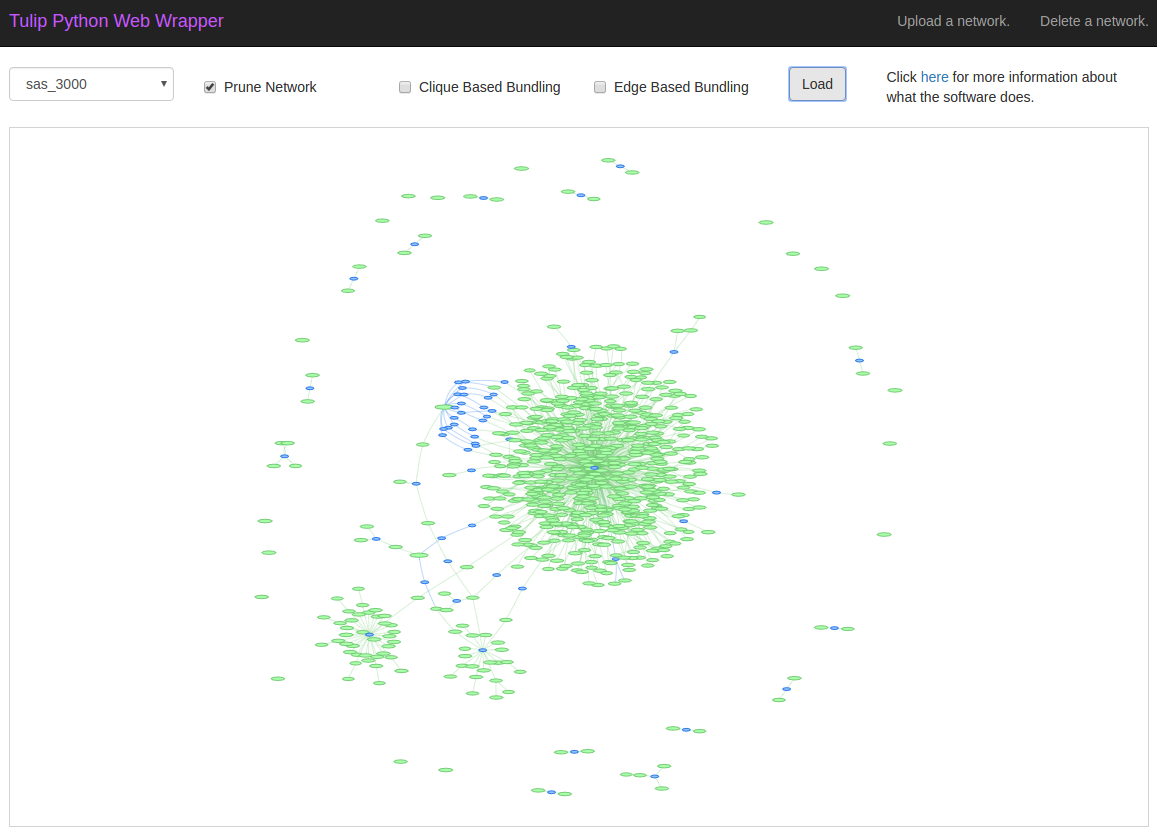
\includegraphics[width=14cm]{appendices/3000_3prune}
    \caption{This shows a network with originally 2849 nodes being rendered after applying node pruning.}
    \label{fig:3000_3prune}
\end{figure}

\begin{figure}[H]
    \centering
    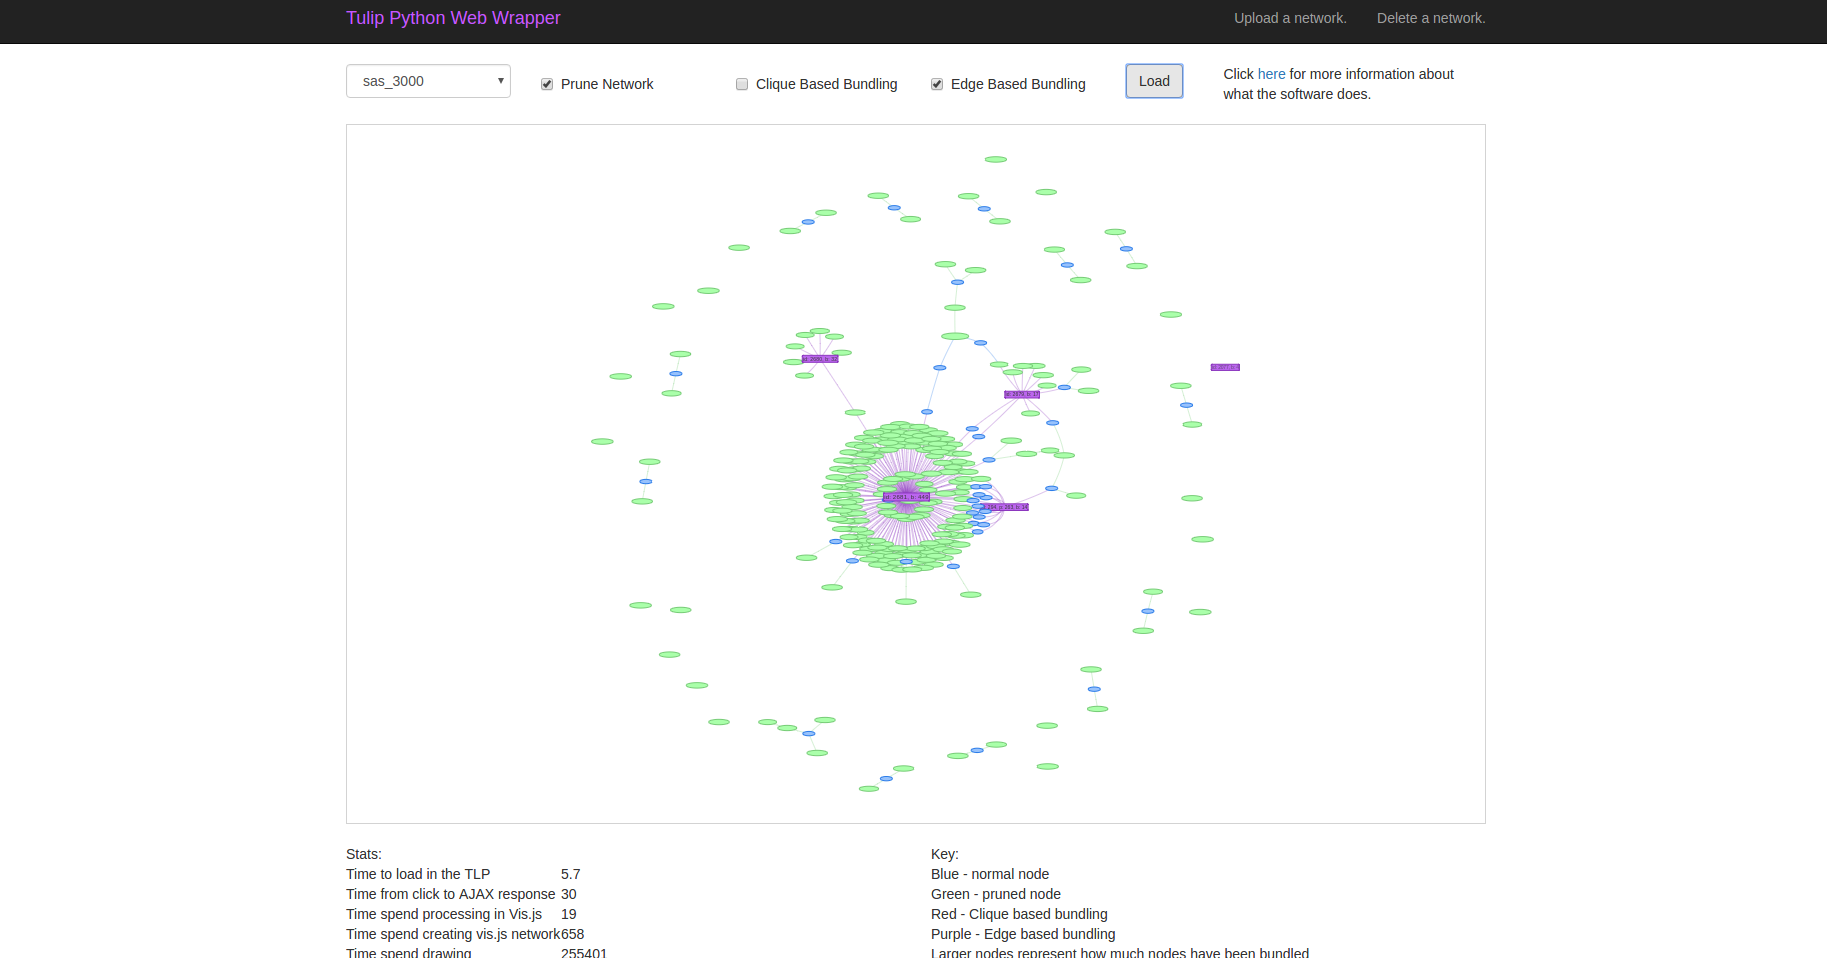
\includegraphics[width=14cm]{appendices/3000_4both}
    \caption{This shows a network with originally 2849 nodes being rendered after applying both node pruning and then node bundling based on number of edges.}
    \label{fig:3000_4both}
\end{figure}

%------------------------------------------------------------

\chapter{How to run and use the System}

\section{Setting up the Django Server}

The server was developed and tested on Linux. Python and Django are both fully supported on Windows and, although virtualenv works slightly differently, Windows compatibility should exist, although it is untested.

In order to run the project, the following steps must be taken:
\begin{enumerate}
    \item \textbf{Ensure Python 3 is installed.} This can be downloaded from https://www.python.org/downloads/. Make sure that, when installing Python, pip (Python Package Index) is also installed. If pip is not installed then it can be by entering: \texttt{sudo apt install python-pip}.
    \item \textbf{Create a virtual environment.} If virtualenv is not installed then open a terminal and enter: \\ \texttt{pip install virtualenv}. Once this has finished installing, a virtual environment is created by navigating to the directory where the virtual environment should be stored and then entering: \\ \texttt{virtualenv tulipwebwrapper --python=python3}. The flag ensures that Python 3 is used if multiple versions of Python exist on the system being used.
    \item \textbf{Activate the virtual environment.} This is done by entering: \\ \texttt{source /path/to/ve/tulipwebwrapper/bin/activate}.
    \item \textbf{Installing the project requirements.} Navigate to the root of the project and then enter the folder named `dev' then `webtulip'. From here, open a terminal and enter: \\ \texttt{pip install -r requirements.txt}.
    \item \textbf{Ensure the database is up to date.} Enter: \texttt{python manage.py makemigrations} to check for and create database migrations (this will have no effect if no models have been changed), and then: \\ \texttt{python manage.py migrate} which will run the migrations and ensure the database schema is up-to-date.
    \item \textbf{Run the server.} Finally, to run the server, just enter: \texttt{python manage.py runserver} (or ./run.sh which contains that exact command.).
\end{enumerate}

In short, once Python 3 and pip are installed, the commands are:
\begin{enumerate}
    \item \texttt{pip install virtualenv}
    \item \texttt{cd path/to/where/ve/should/be/created}
    \item \texttt{virtualenv tulipwebwrapper --python=python3}
    \item \texttt{source /path/to/ve/tulipwebwrapper/bin/activate}
    \item \texttt{cd path/to/project/dev/webtulip}
    \item \texttt{pip install -r requirements.txt}
    \item \texttt{python manage.py makemigrations}
    \item \texttt{python manage.py migrate}
    \item \texttt{python manage.py runserver}
\end{enumerate}

\section{Accessing and using the interface}

Once the server is running, navigating to \texttt{http://127.0.0.1:8000} in any browser will direct users to the home page of the system.

From here, users can navigate to the upload page (\texttt{http://127.0.0.1:8000/upload}) and upload networks into the system. The system accepts \texttt{.tlp} networks and \texttt{.json} networks in the format that SAS use. Examples of these can be found in /path/to/project/data/sas\_data, which contains two folders, one containing the \texttt{.tlp}'s (previously converted) and one containing the original \texttt{.json} files. Additionally, in the project/data folder, there is g1.tlp and g2.tlp, two very simple networks which were used for testing. To upload a \texttt{.tlp}, set the network type to `Tulip TLP' (default) and to upload a \texttt{.json}, set the network type to `Industry Standard'. 

Once network(s) have been uploaded, navigate back to the home page and from there, select the network to visualise and then select any algorithms to be applied to the network.

\end{appendices}
